% !TeX root = document.tex
% !TeX encoding = UTF-8 Unicode

\chapter{Resposta do Sistema}%
\label{chapter:system-response}

Nesse módulo são feitas as configurações de teste em malha aberta. O nome do
módulo remete ao fato que ele permite obter a resposta do sistema à um sinal de
entrada. Na Figura~\ref{fig:system-response1} pode-se ver a lista de testes
configurados, bem como as opções de gerenciar tais testes.

\begin{figure}[ht!]
    \centering
    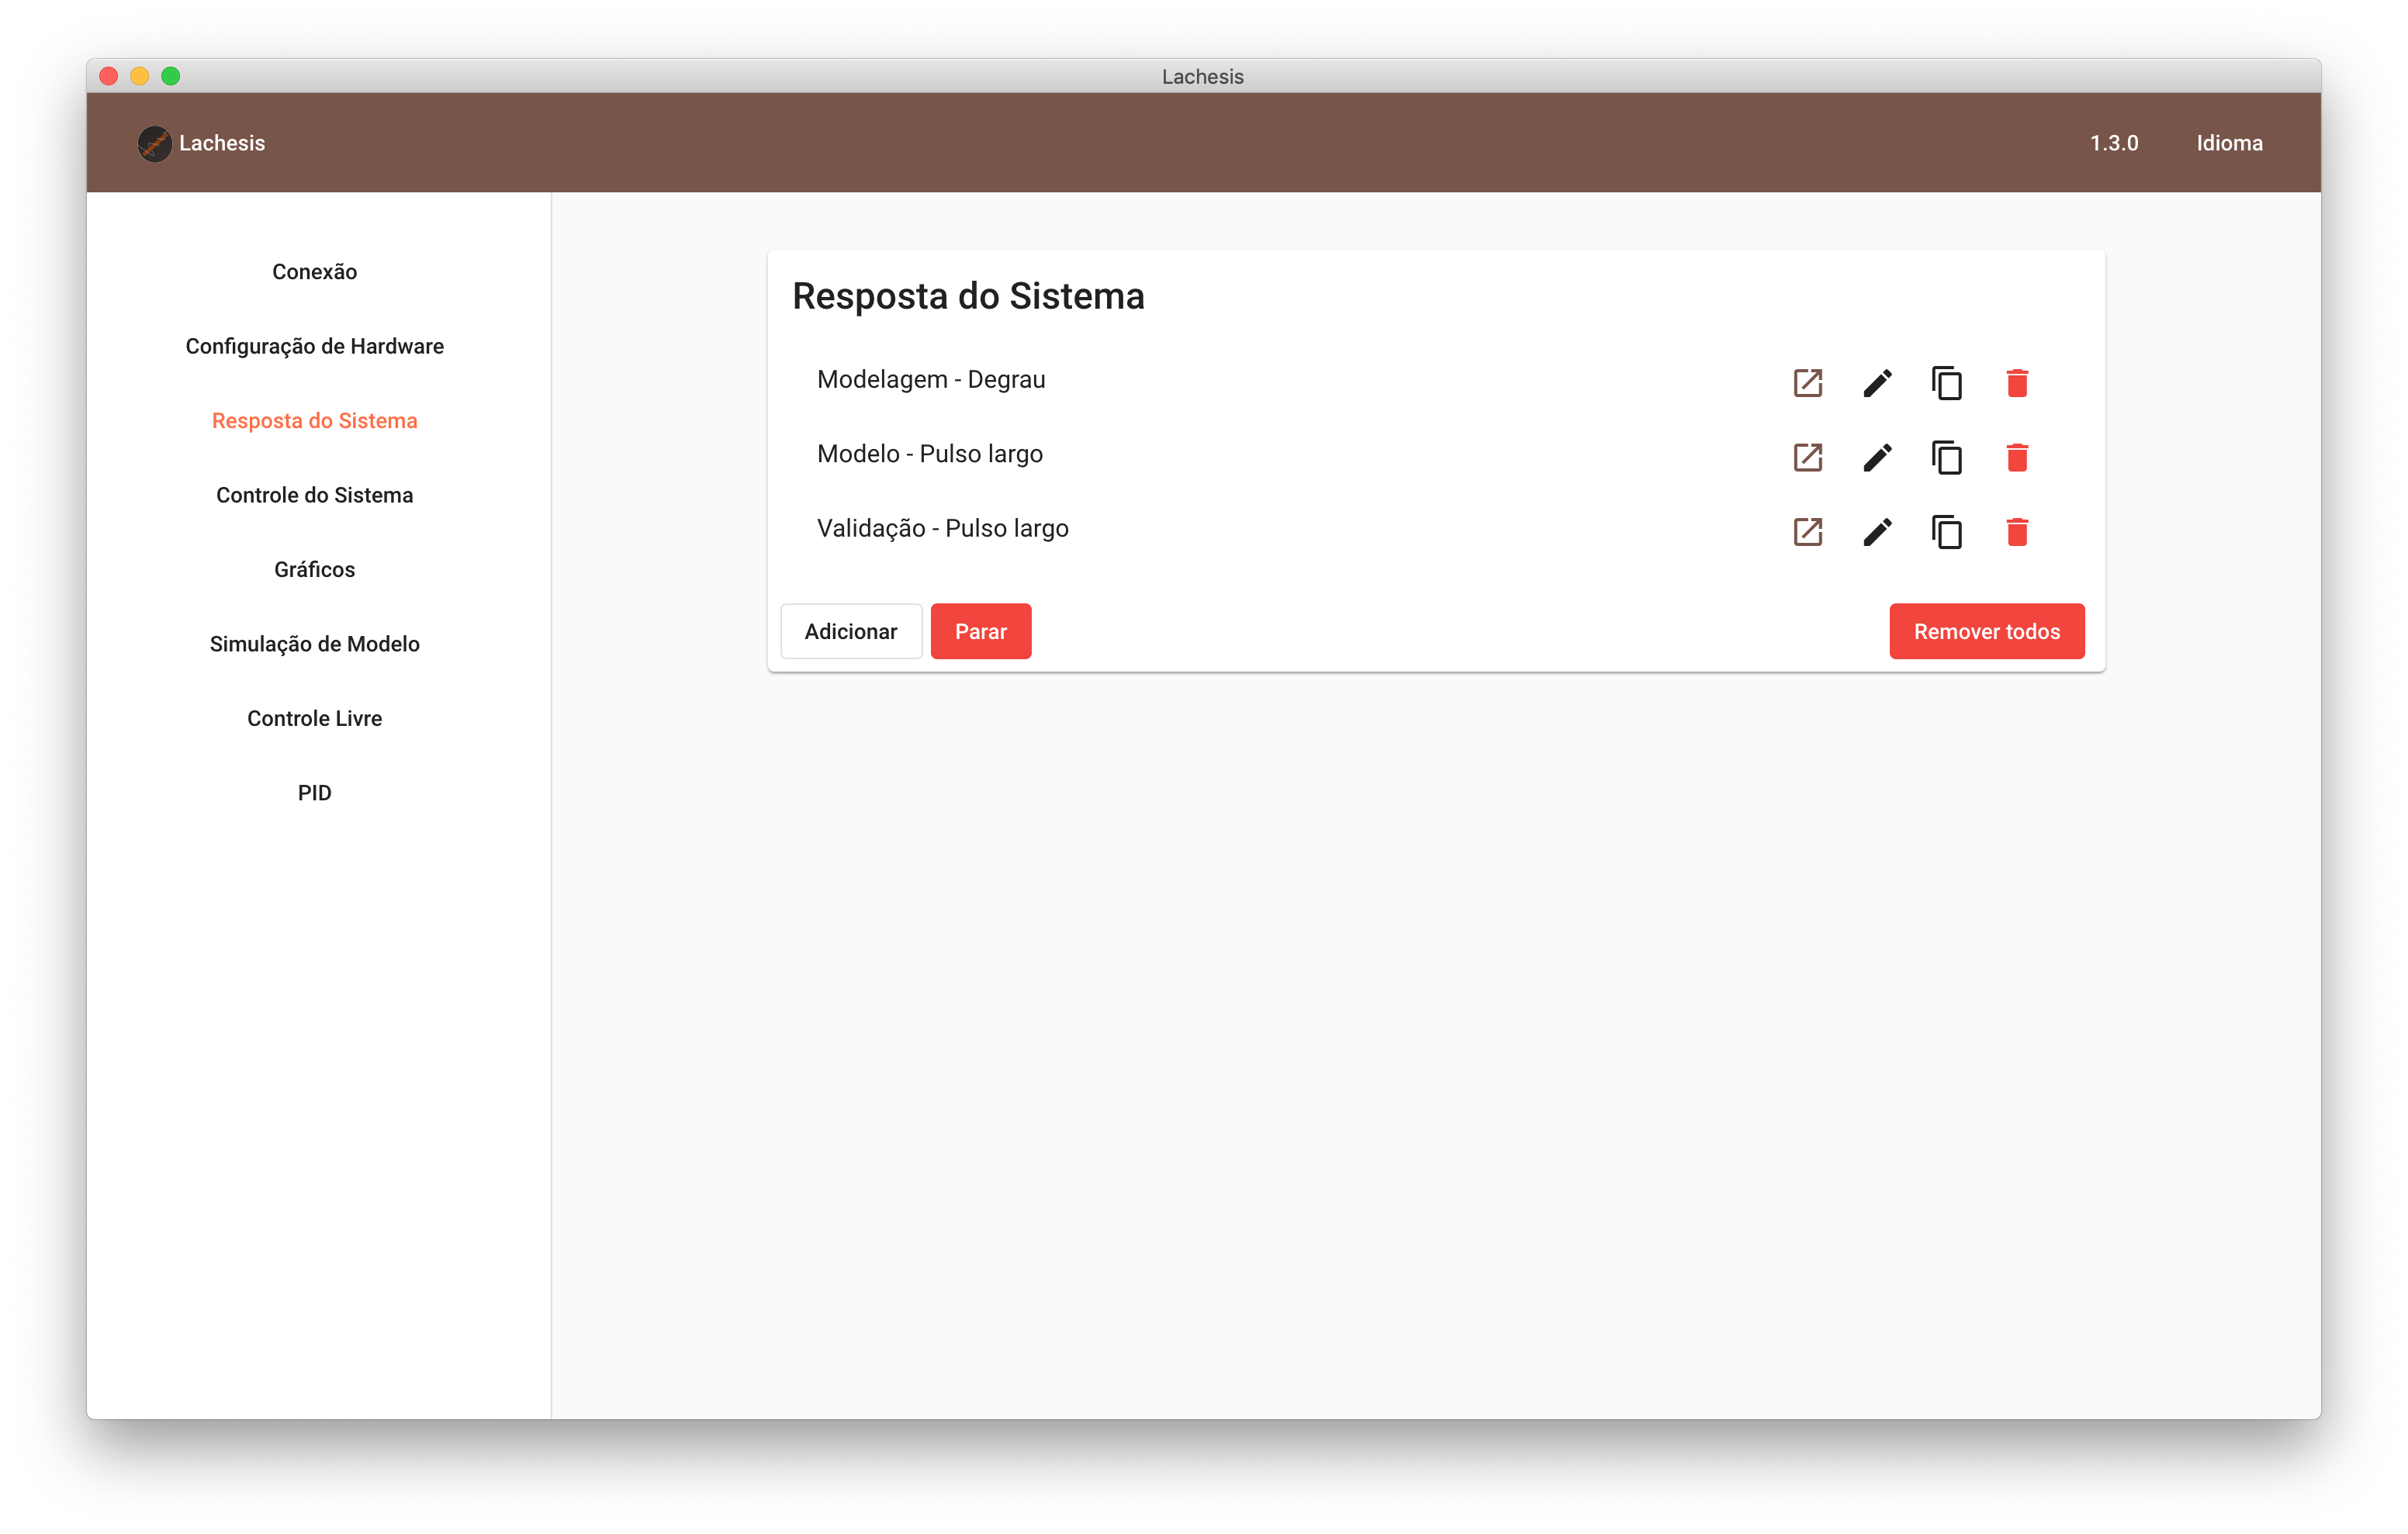
\includegraphics[width=0.9\textwidth]{imgs/system-response1}
    \caption[Módulo Resposta do Sistema]{Módulo Resposta do Sistema}%
    \label{fig:system-response1}
\end{figure}

O botão \textit{Clonar} cria uma cópia do teste. Essa opção é útil para criar
vários testes que possuem apenas pequenas diferenças entre si. O botão
\textit{Executar} inicia o teste e navega para o módulo \textit{Gráficos}. O
botão \textit{Parar} irá interromper \textbf{qualquer} teste que esteja em
execução, não importa o tipo.

Ao adicionar ou editar um teste é possível criar um sinal facilmente, apenas
preenchendo um formulário. Várias formas de onda estão disponíveis para
preenchimento rápido. Cada opção será detalhada nas seções a seguir. Algumas
configurações são comuns e serão tratadas na seção~\ref{sec:step}.

\section{Degrau}%
\label{sec:step}

Todo teste tem um nome. O nome do teste, juntamente com sua data de execução,
serão exibidos na lista de gráficos, onde pode-se ver os gráficos e exportar os
dados (Ver Capítulo~\ref{chapter:graficos}). Portanto, escolha um nome que
permita identificar o motivo de tal teste ter sido realizado e/ou os parâmetros
que foram usados em sua execução. Em um ambiente onde mais de uma pessoa utiliza
o mesmo sistema, também é boa prática colocar seu nome no teste.

Na aba \textit{Degrau}, mostrada na Figura~\ref{fig:system-response2}, é
possível definir um sinal desse tipo. Para isso deve-se informar o valor inicial
\textit{\(V_0\)}, o acréscimo \textit{\(\Delta{}V\)}, que será somado ao valor
inicial após \textit{\(T_0\)} segundos, e o tempo \textit{\(T_1\)} que o sinal
\textit{\(V_0 + \Delta{}V\)} ficará aplicado.

\begin{figure}[ht!]
    \centering
    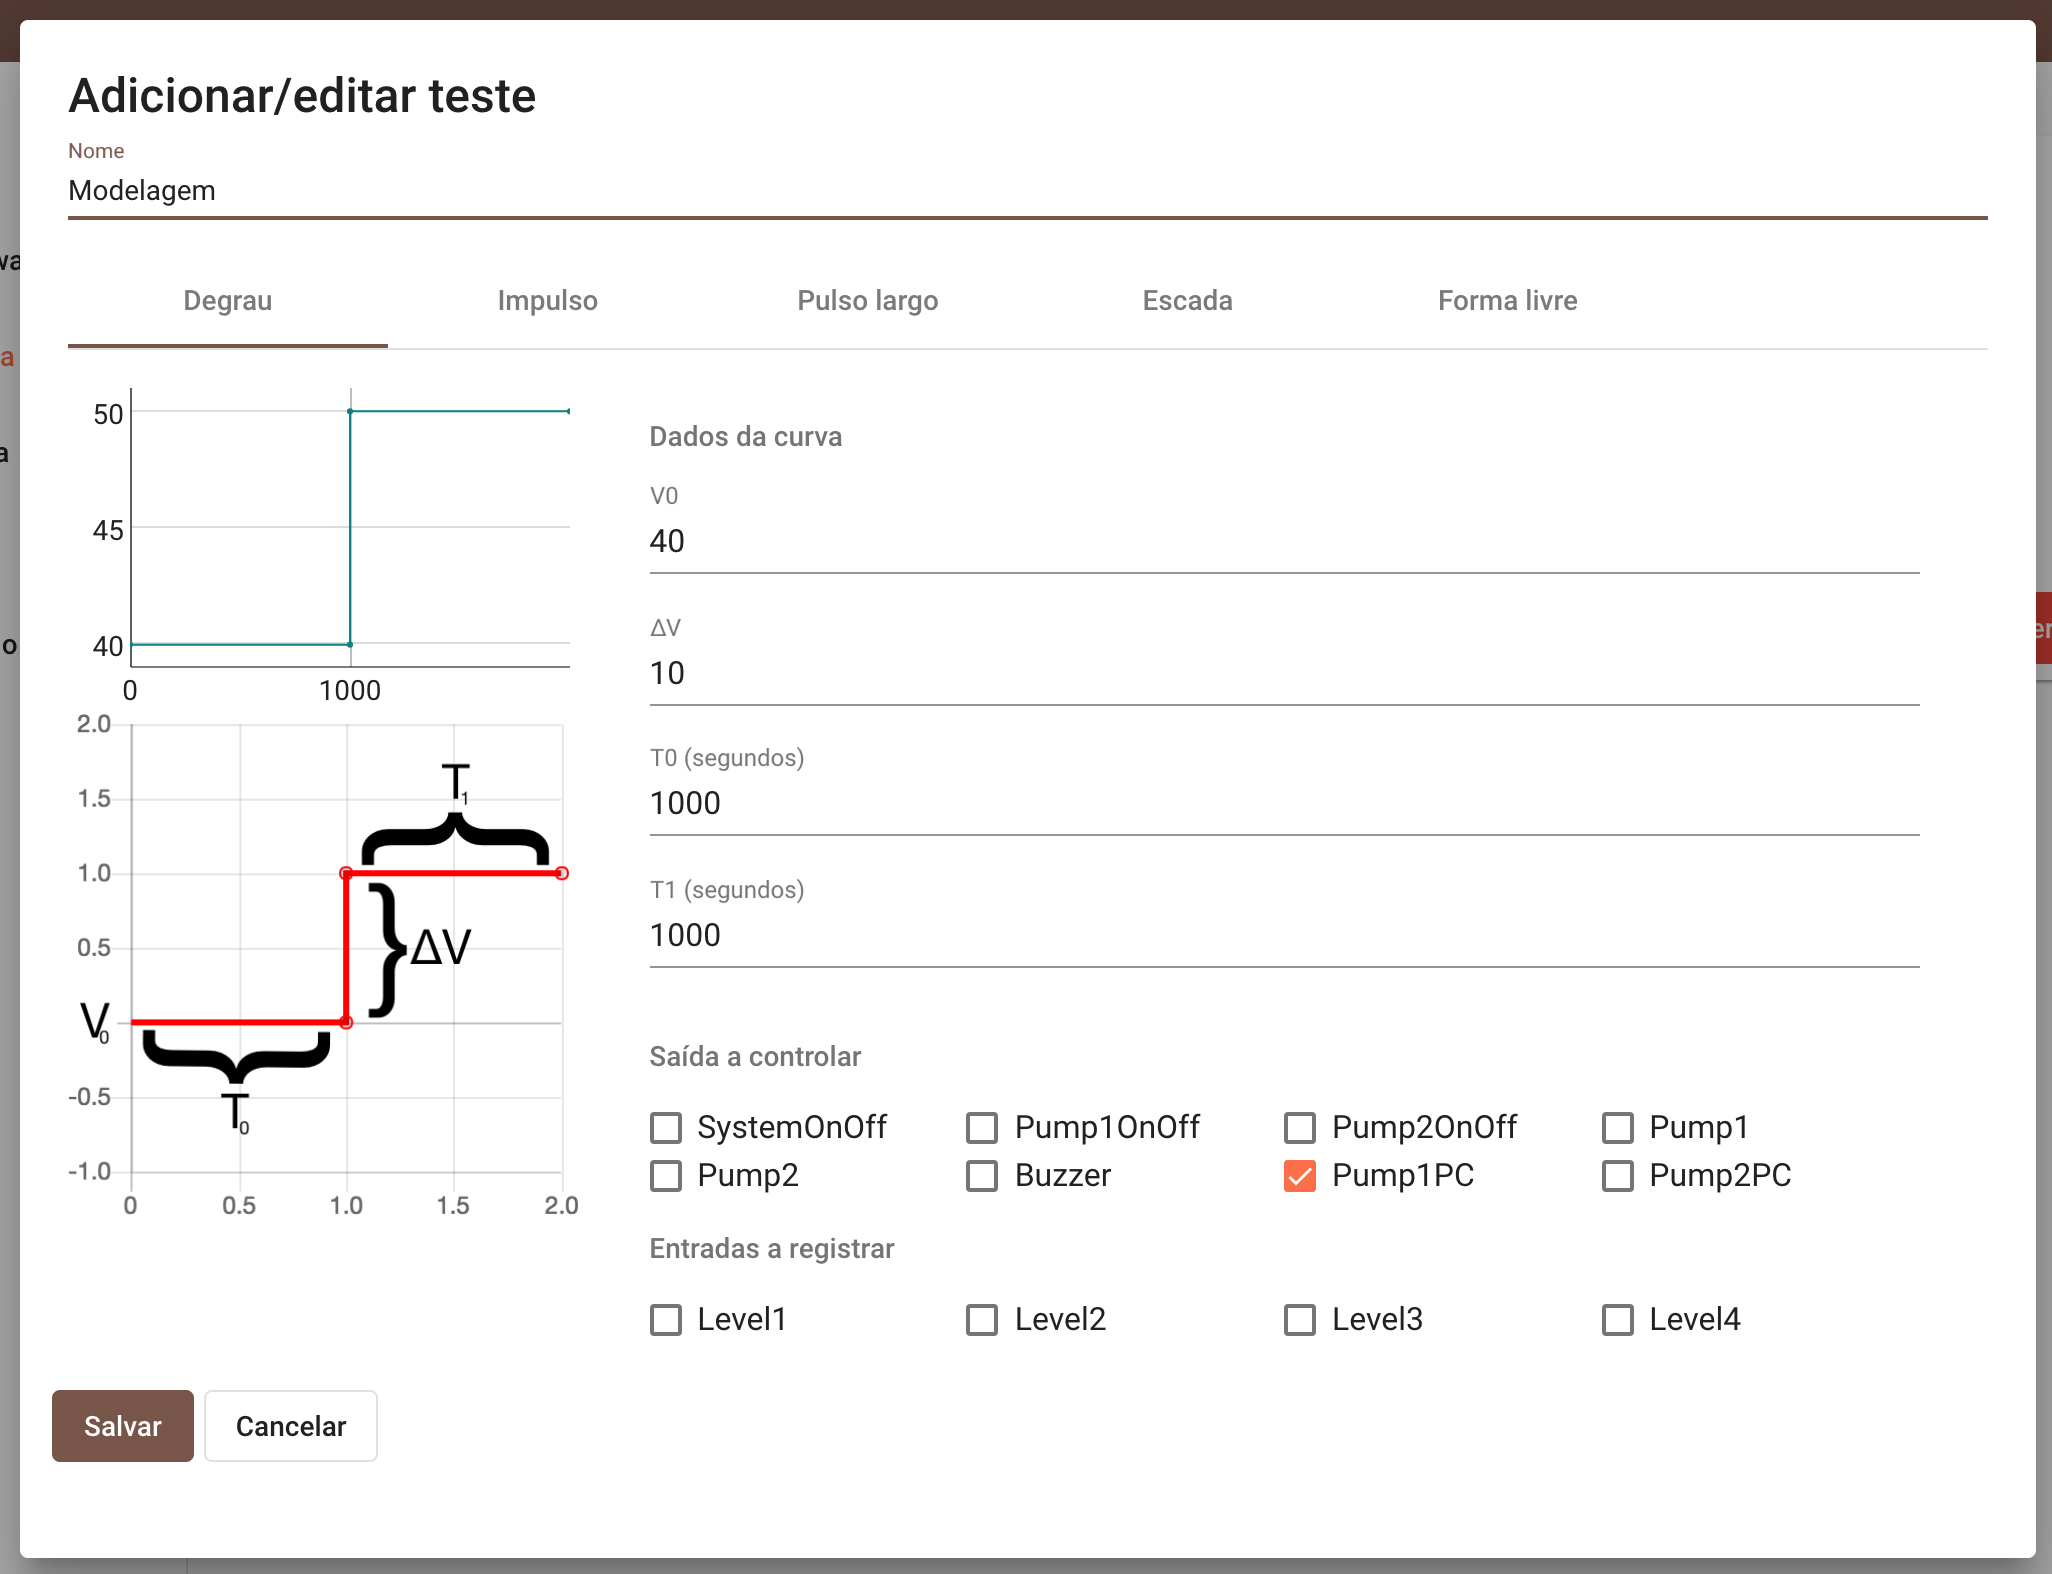
\includegraphics[width=0.9\textwidth]{imgs/system-response2}
    \caption[Sinal do tipo degrau]{Sinal do tipo degrau}%
    \label{fig:system-response2}
\end{figure}

A seção \textit{Configuração de entrada/saída} permite escolher em quais
atuadores o sinal descrito será aplicado. É possível escolher mais de um
atuador, mas todos receberam o mesmo sinal. Também deve-se escolher quais
entradas serão registradas, como mostrado na Figura~\ref{fig:system-response3}.

\begin{figure}[ht!]
    \centering
    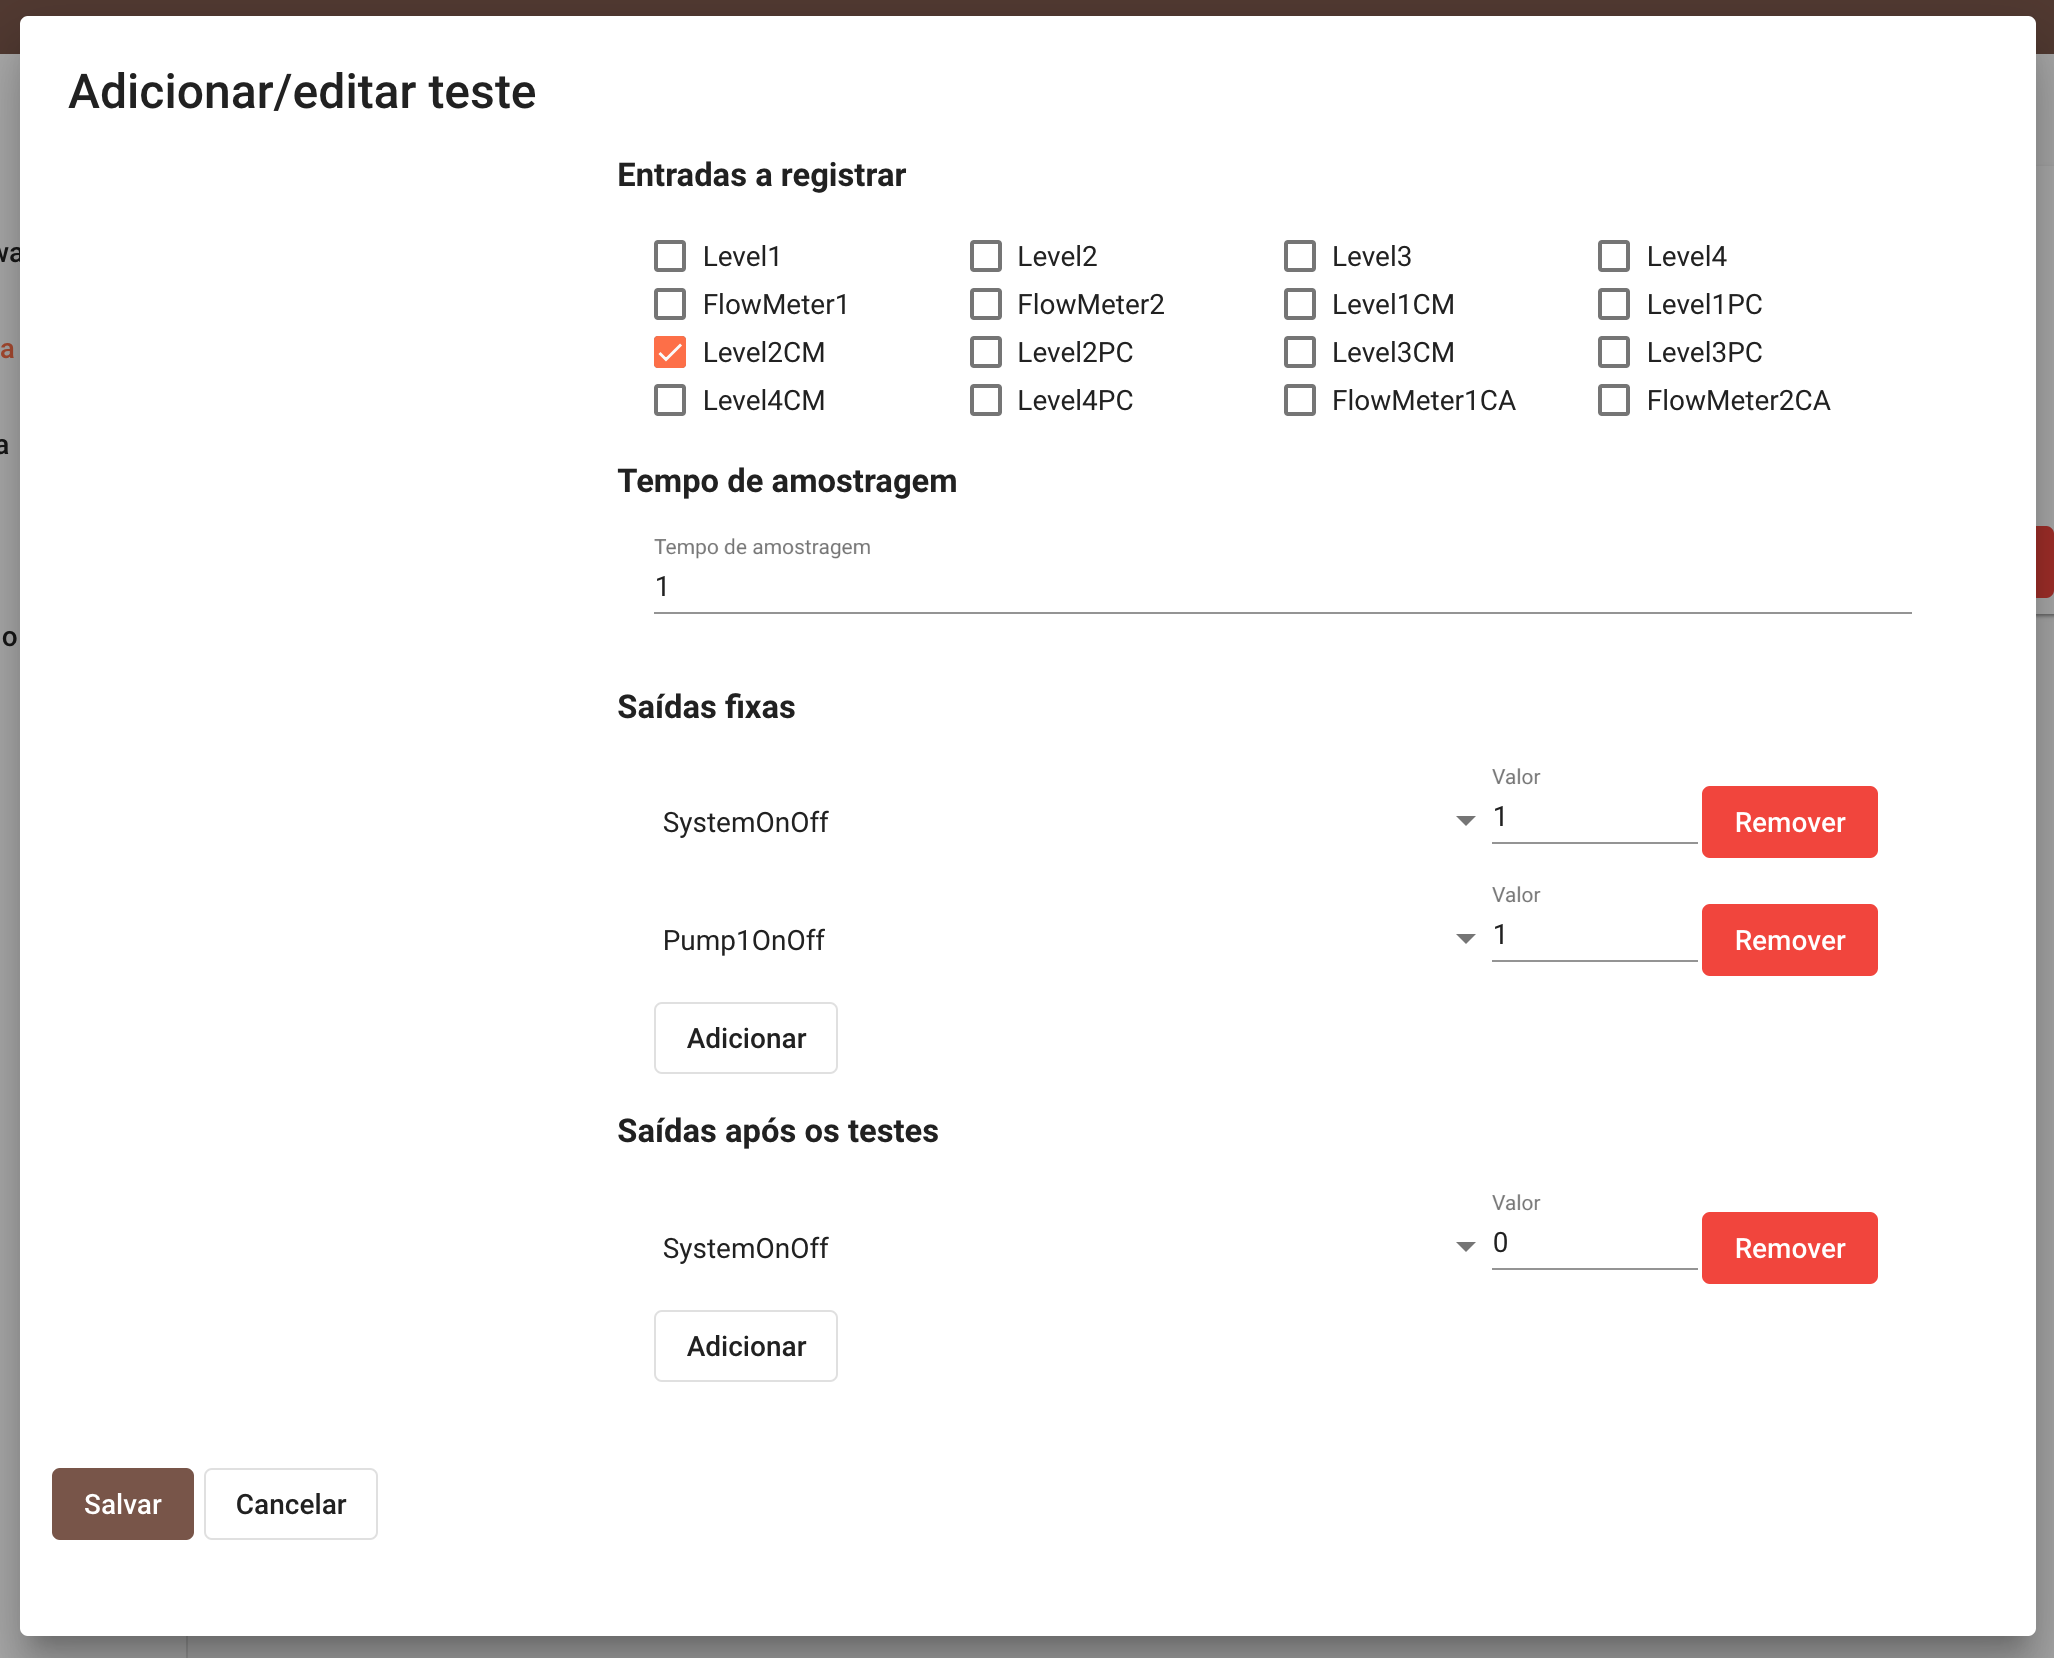
\includegraphics[width=0.9\textwidth]{imgs/system-response3}
    \caption[Configuração comum]{Configuração comum}%
    \label{fig:system-response3}
\end{figure}

\textit{Tempo de amostragem} é o tempo entre cada leitura dos sensores. Os
atuadores também serão atualizados apenas após passado esse tempo desde a
última atualização.

\textit{Saídas fixas} são portas que terão seus valores escritos antes do teste
iniciar. Seu principal objetivo é permitir definir valores de portas que atuam
como chave geral do sistema. Da mesma forma \textit{Saídas após o teste} serão
definidas após o teste terminar, ou caso algum erro ocorra durante a execução,
como, por exemplo, o acionamento de um intertravamento.

\newpage{}
\section{Impulso}%
\label{sec:impulse}

Nessa aba pode-se definir um sinal do tipo impulso discreto. Deve-se definir as
durações e o valor inicial, mas não a variação da amplitude, como no caso do
sinal degrau. Essa amplitude será calculada de forma a fazer com que o gráfico
do sinal tenha área 1 na região sob \(\Delta{}T\).

\begin{figure}[ht!]
    \centering
    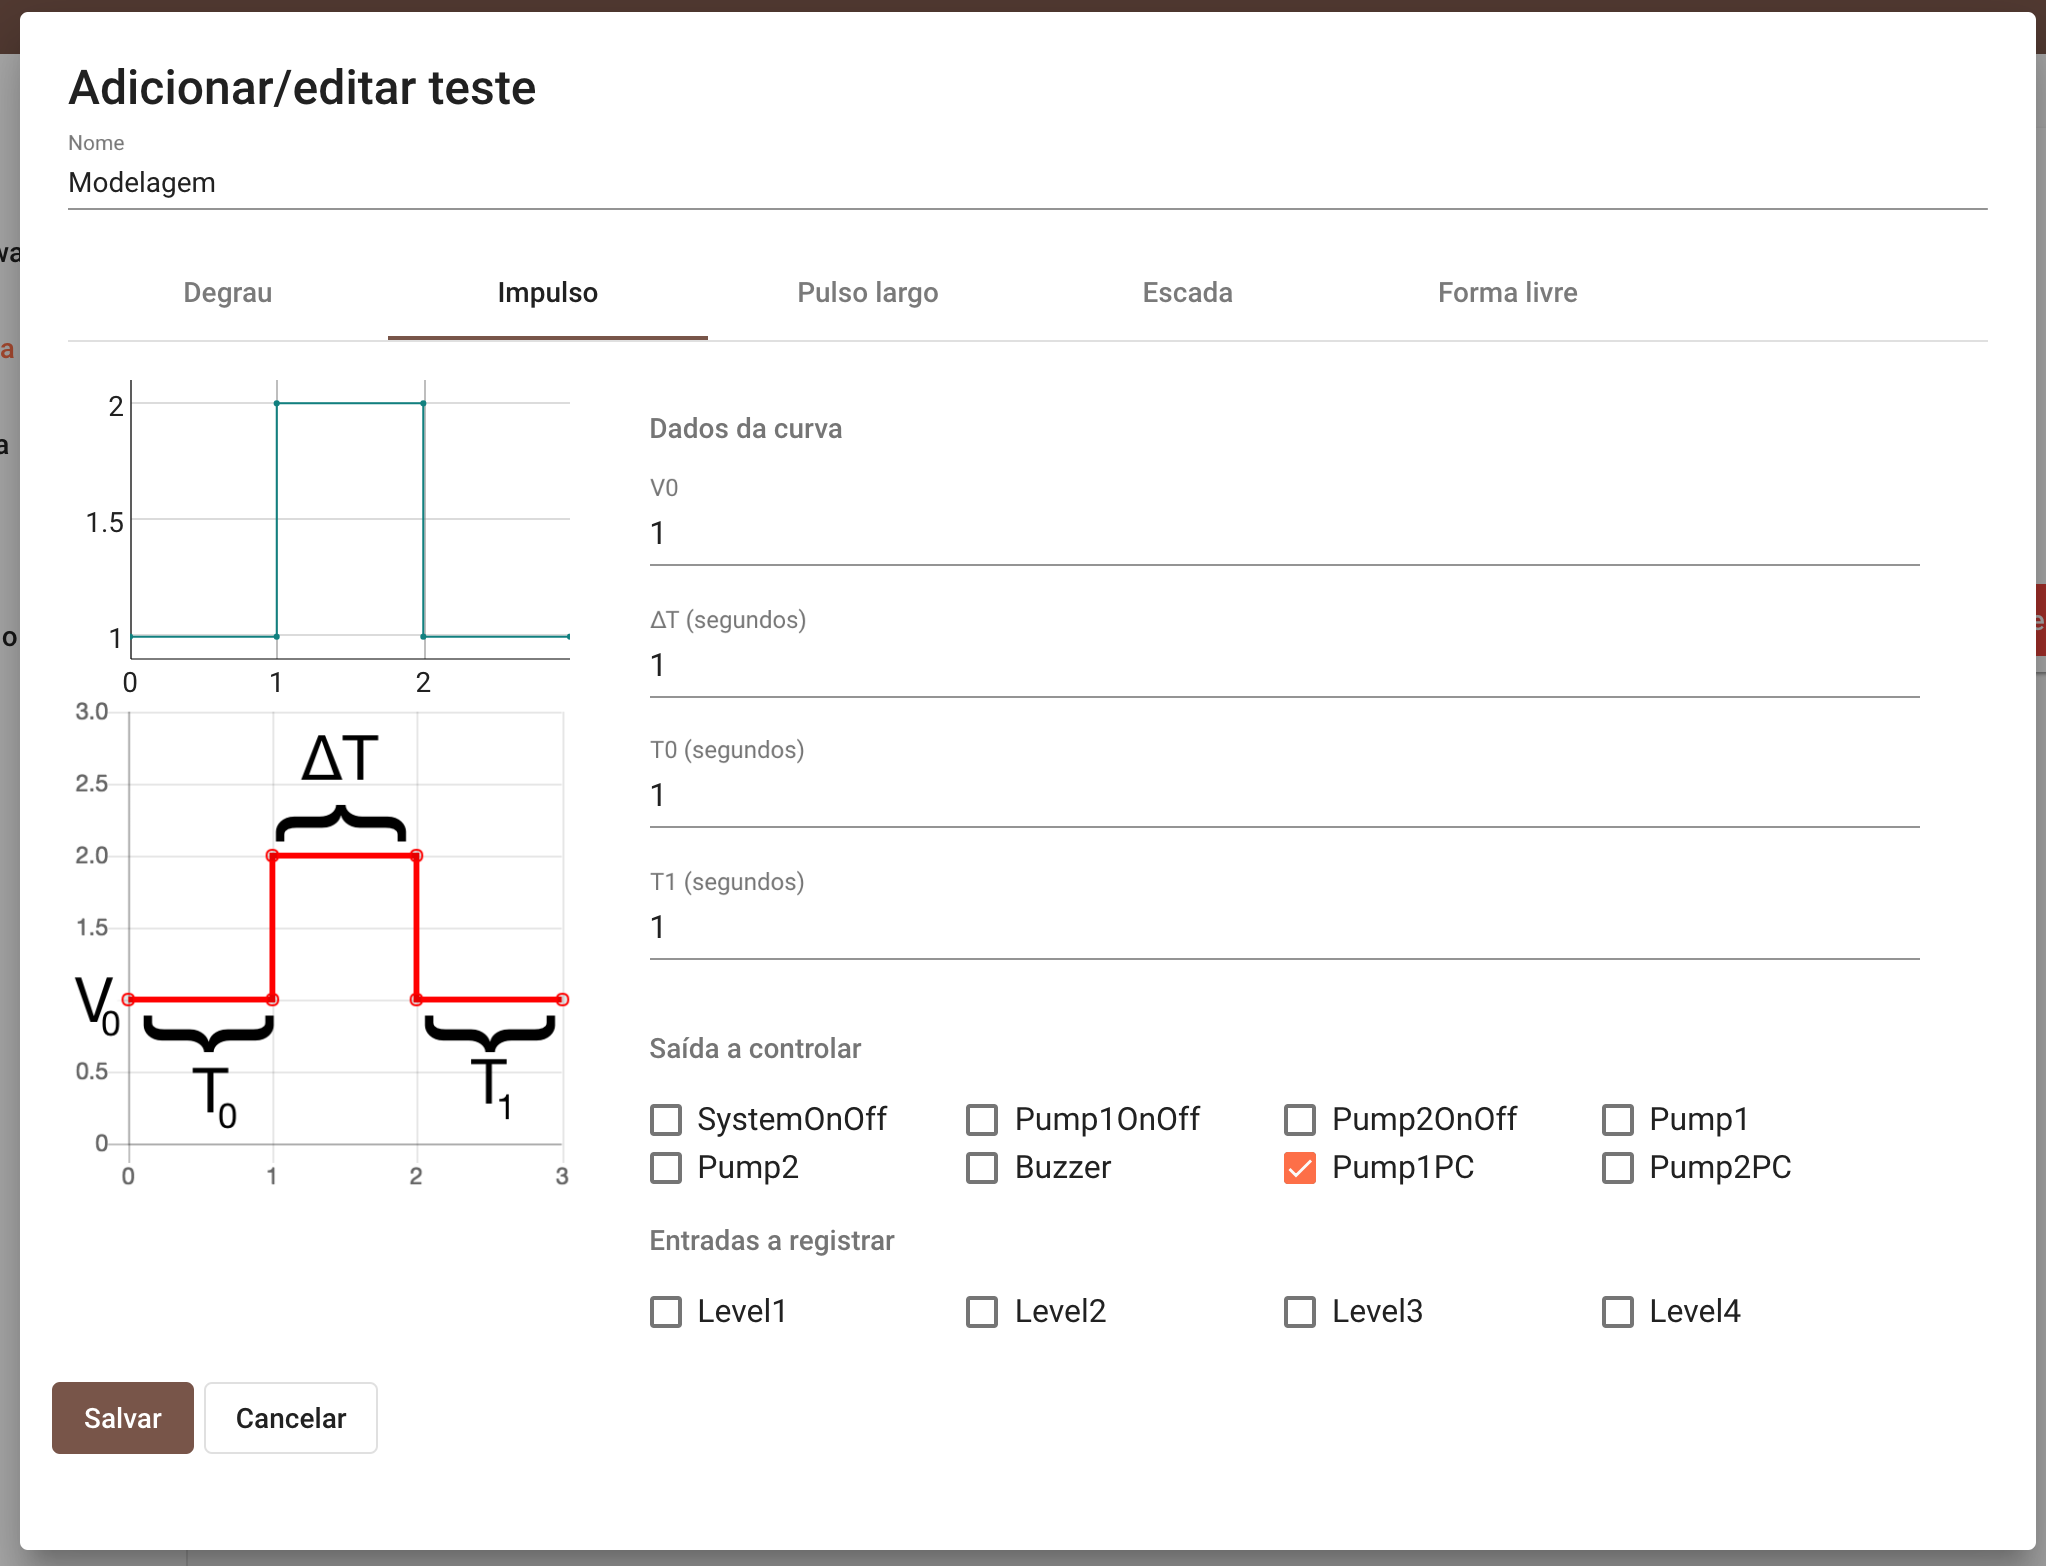
\includegraphics[width=0.9\textwidth]{imgs/system-response4}
    \caption[Impulso]{Impulso}%
    \label{fig:system-response4}
\end{figure}

\newpage{}
\section{Pulso largo}%
\label{sec:wide-pulse}

Parecido com o sinal do tipo degrau, porém deve-se definir um segundo acréscimo
e duração, fazendo com que esse sinal seja a composição de dois sinais do tipo
degrau.

\begin{figure}[ht!]
    \centering
    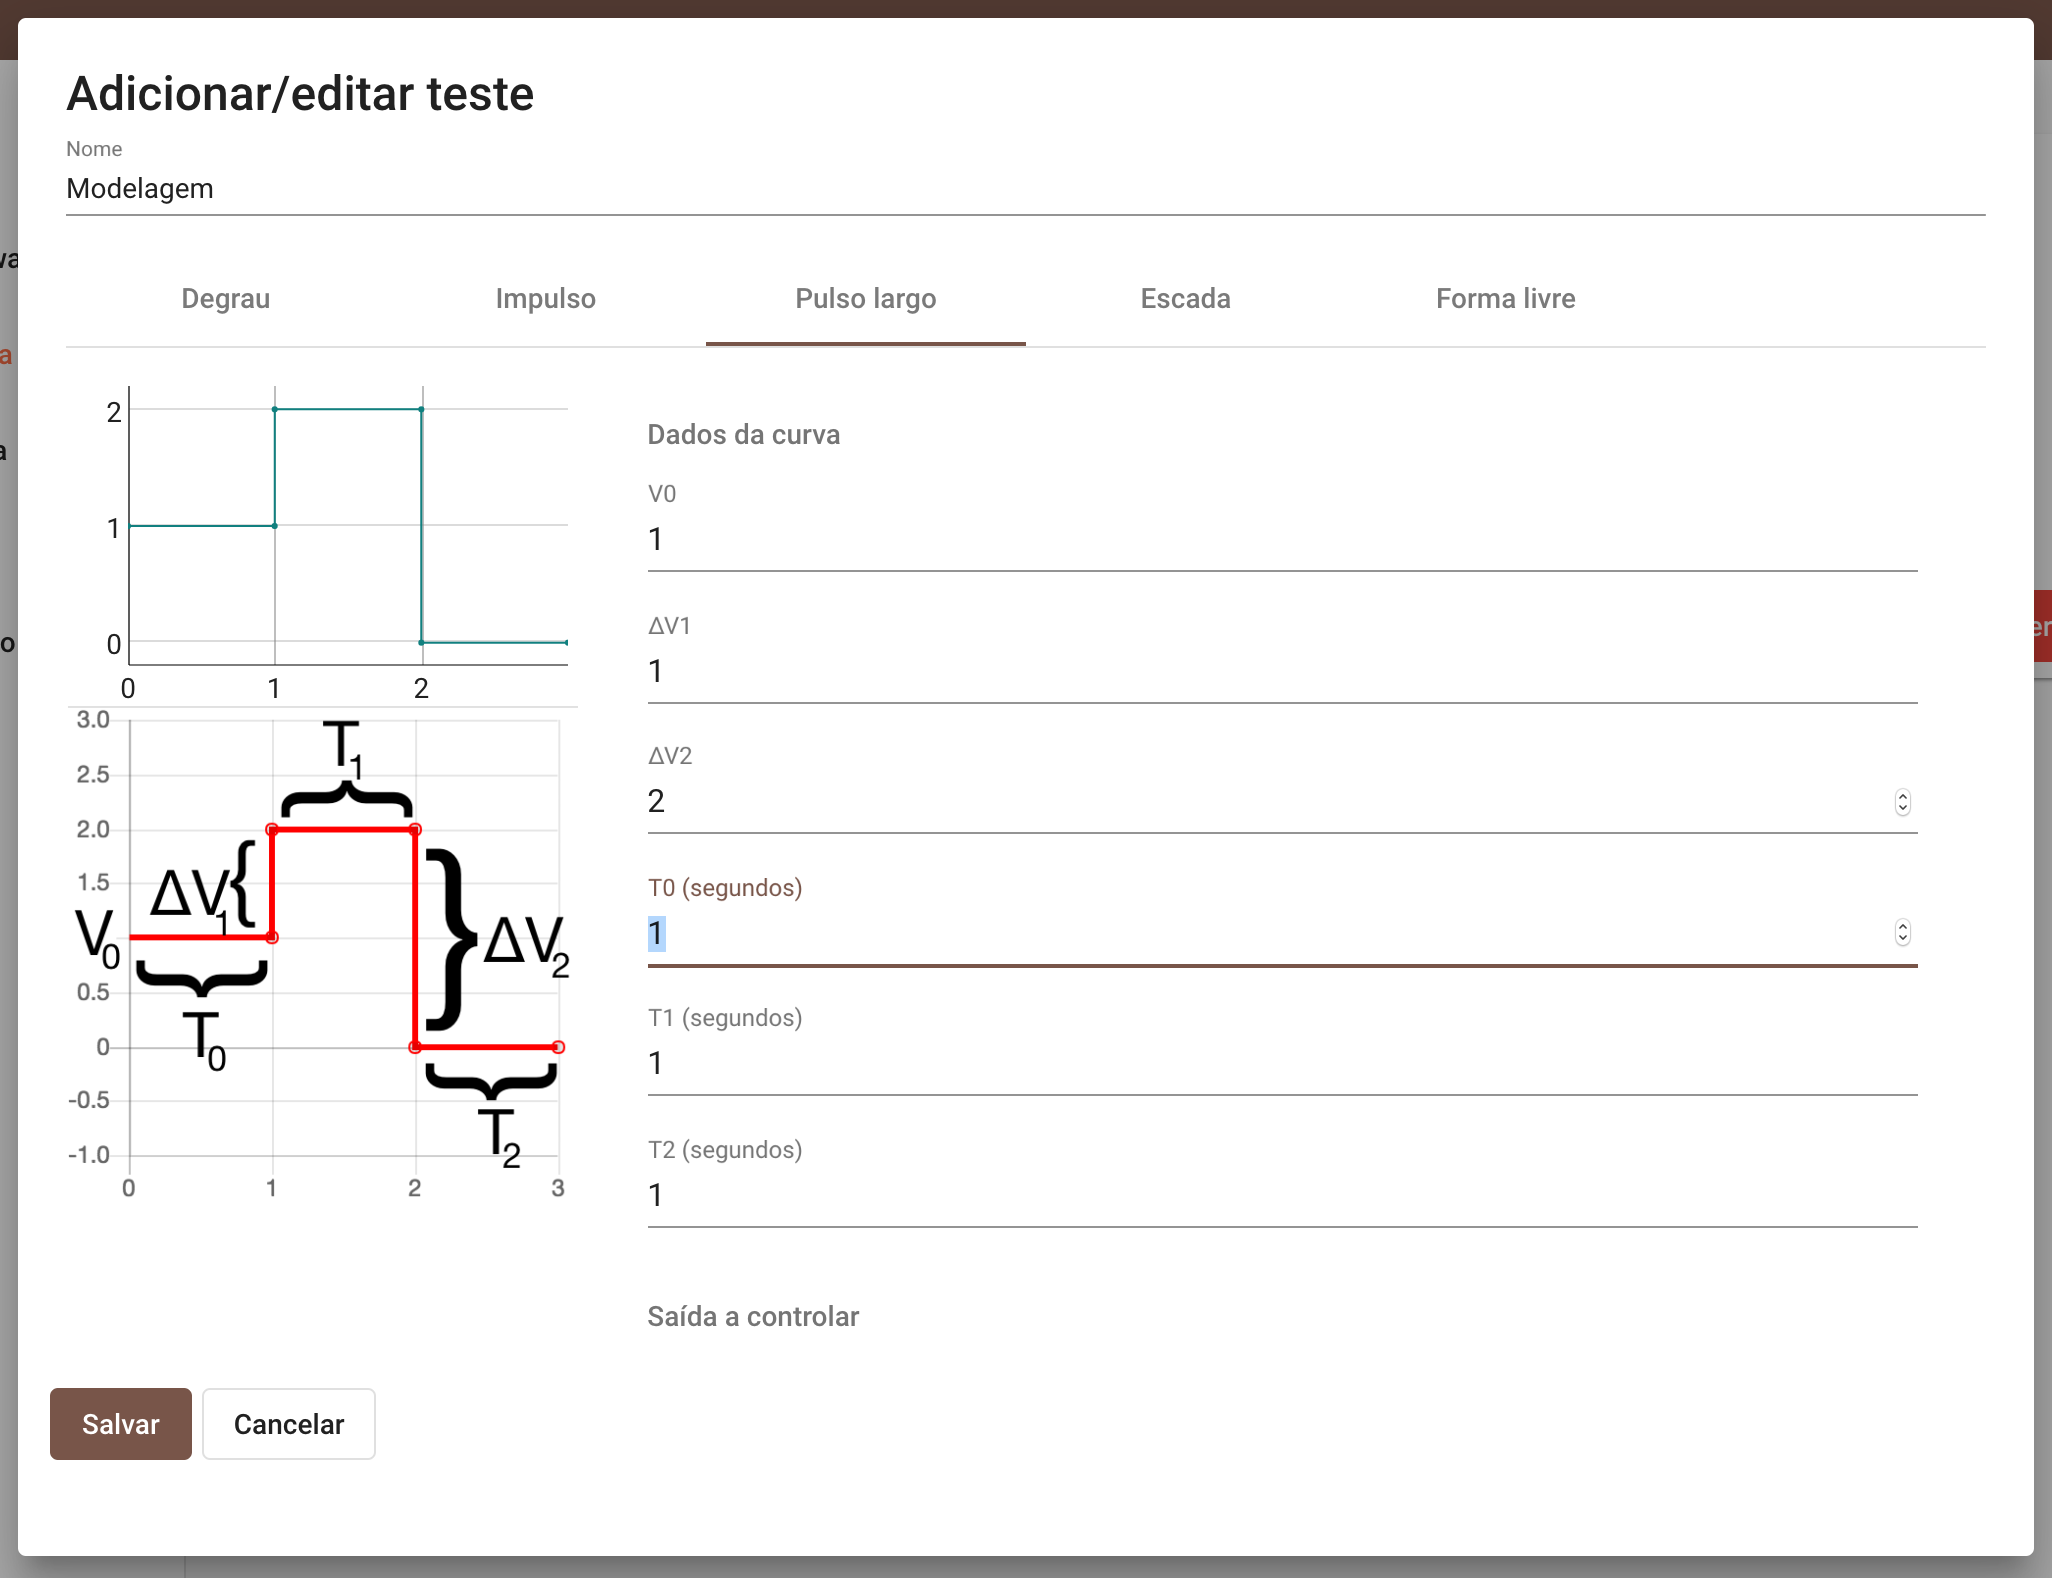
\includegraphics[width=0.9\textwidth]{imgs/system-response5}
    \caption[Pulso largo]{Pulso largo}%
    \label{fig:system-response5}
\end{figure}

\newpage{}
\section{Escada}%
\label{sec:stairs}

Permite a configuração simples de um sinal do tipo escada. Basta informar os
valores incial e final, o número de degraus e a duração de cada degrau.

\begin{figure}[ht!]
    \centering
    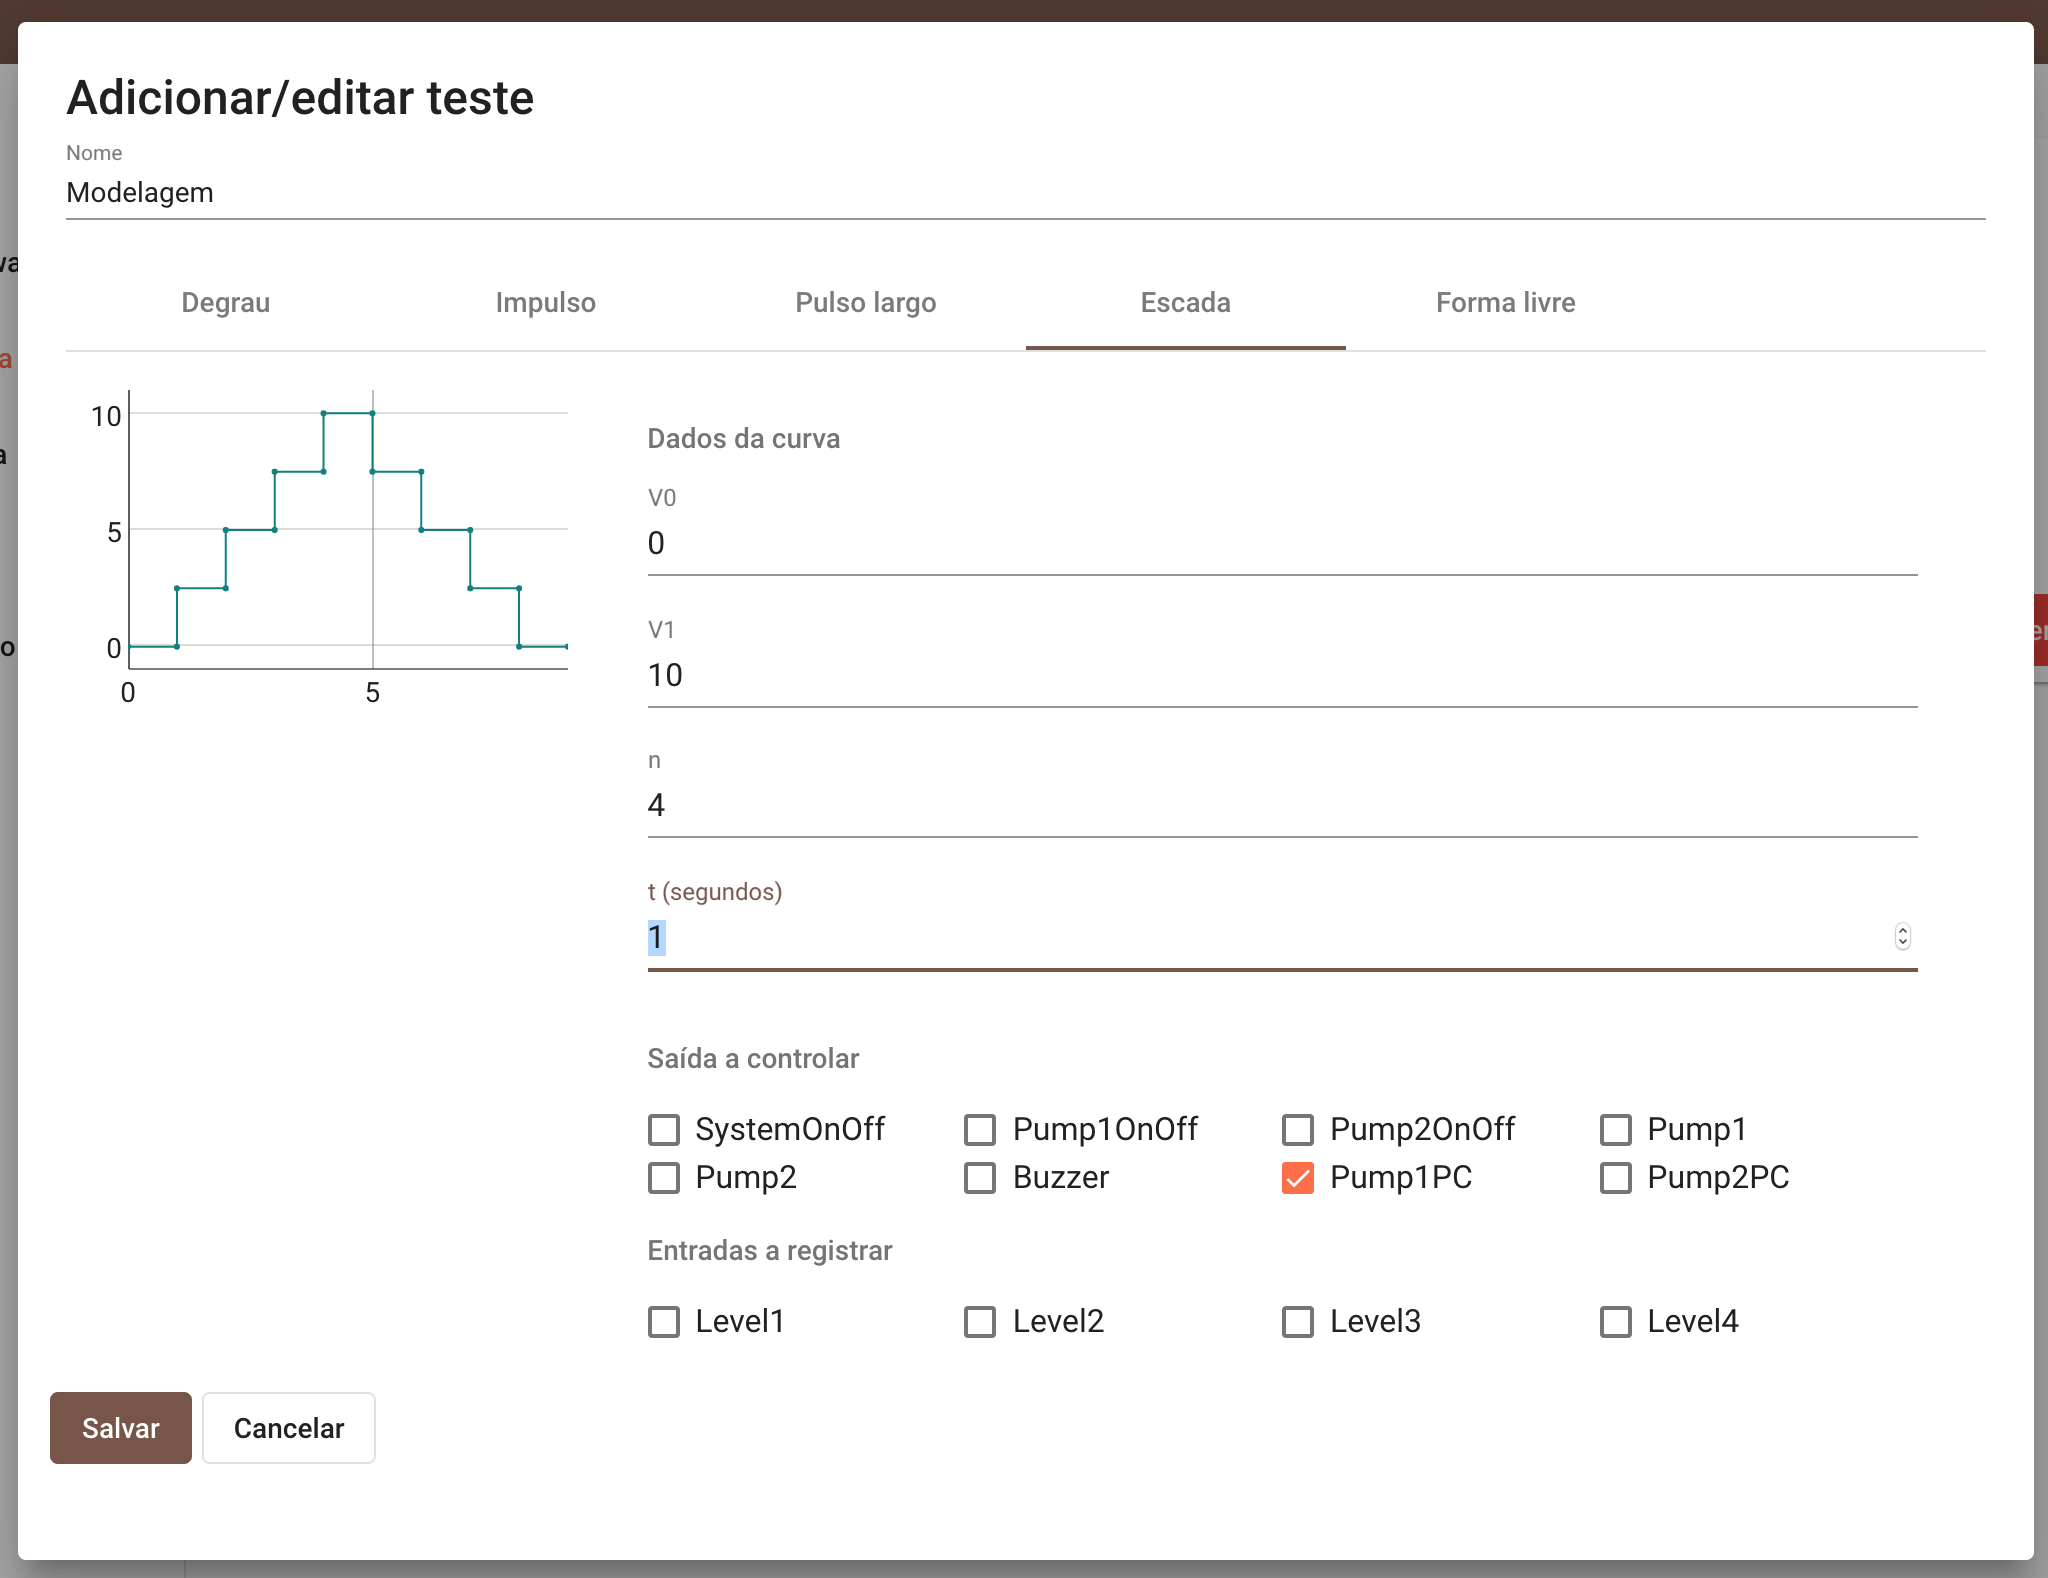
\includegraphics[width=0.9\textwidth]{imgs/system-response6}
    \caption[Escada]{Escada}%
    \label{fig:system-response6}
\end{figure}

\newpage{}
\section{Forma livre}%
\label{sec:free-form}

Nessa aba o sinal pode ser construído ponto a ponto. Também é possível importar
dados de outros aplicativos nos formatos \textit{JSON} e \textit{CSV}. No caso
do \textit{JSON} os dados devem ser no formato \mintinline{javascript}{[{"x": 0,
"y": 0}, {"x": 1, "y": 1}]}. Caso seja usado \textit{CSV}, o tempo deve vir na
primeira coluna e a amplitude na segunda.

O comando \mintinline{matlab}{csvwrite("data.csv", transpose([x; y]))} pode ser
usado para transformar vetores de valores em \textit{CSV}. Após executar esse
comando um arquivo como o nome \textit{data.csv} será criado. Basta abri-lo com
um editor de texto e copiar o conteúdo para a caixa e clicar em
\textit{Importar}.

\begin{figure}[ht!]
    \centering
    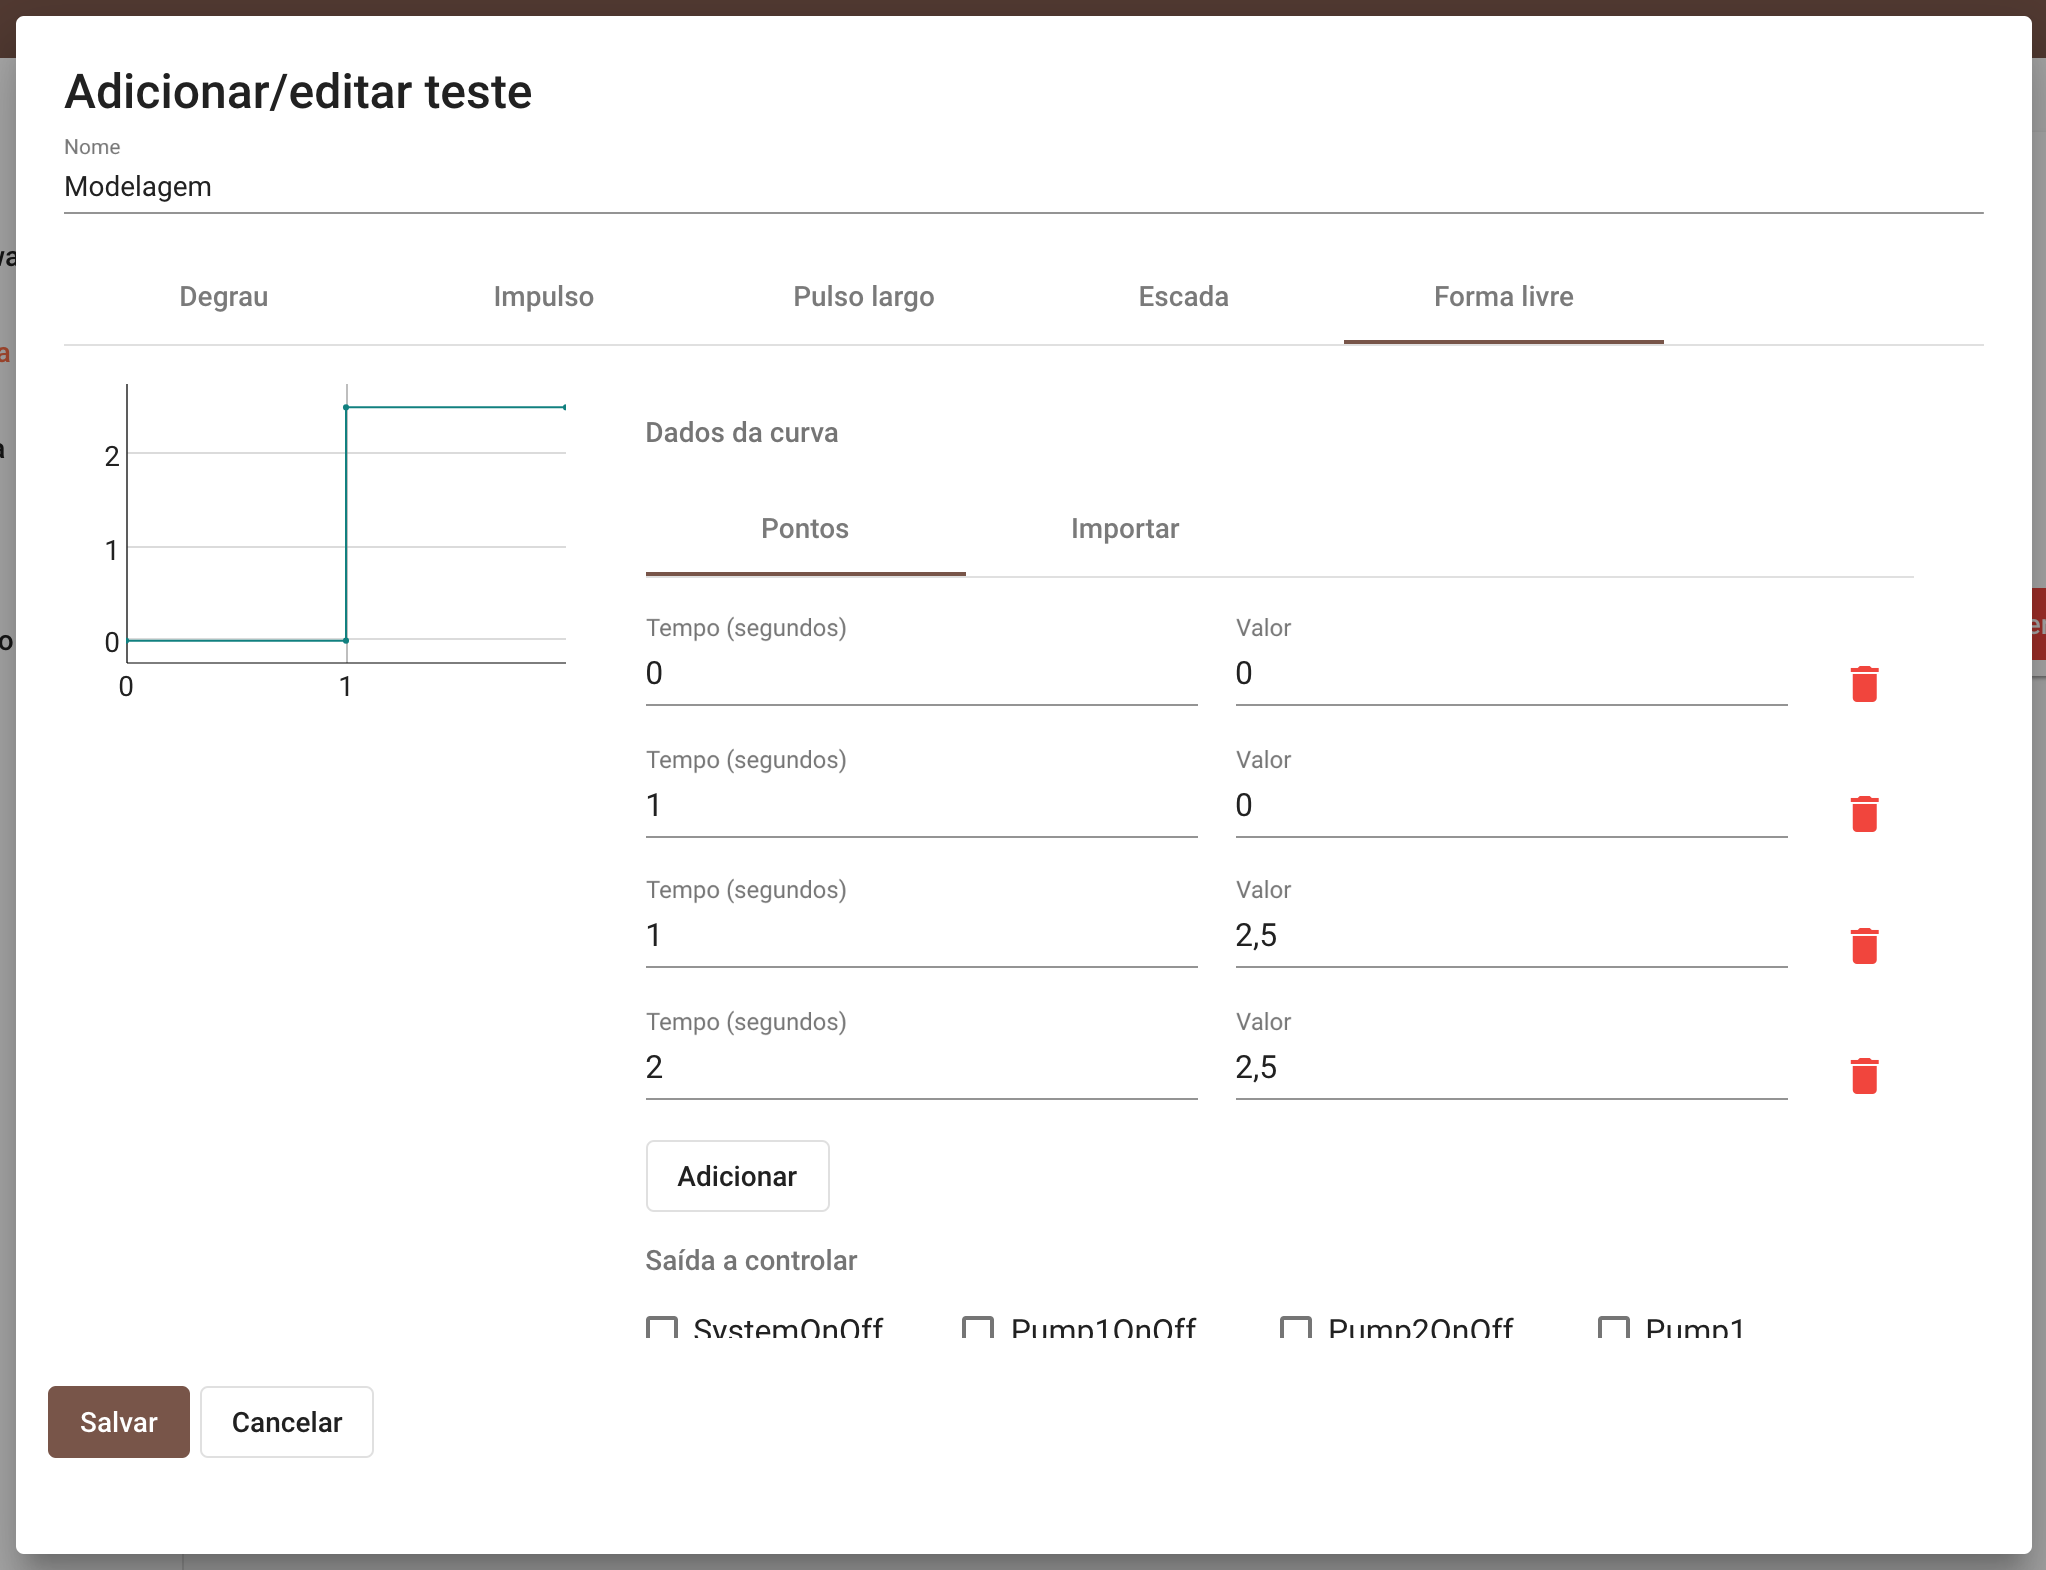
\includegraphics[width=0.9\textwidth]{imgs/system-response7}
    \caption[Forma livre]{Forma livre}%
    \label{fig:system-response7}
\end{figure}
